\renewcommand{\baselinestretch}{1.25}%
\begin{figure}[!t]%
  \centering
  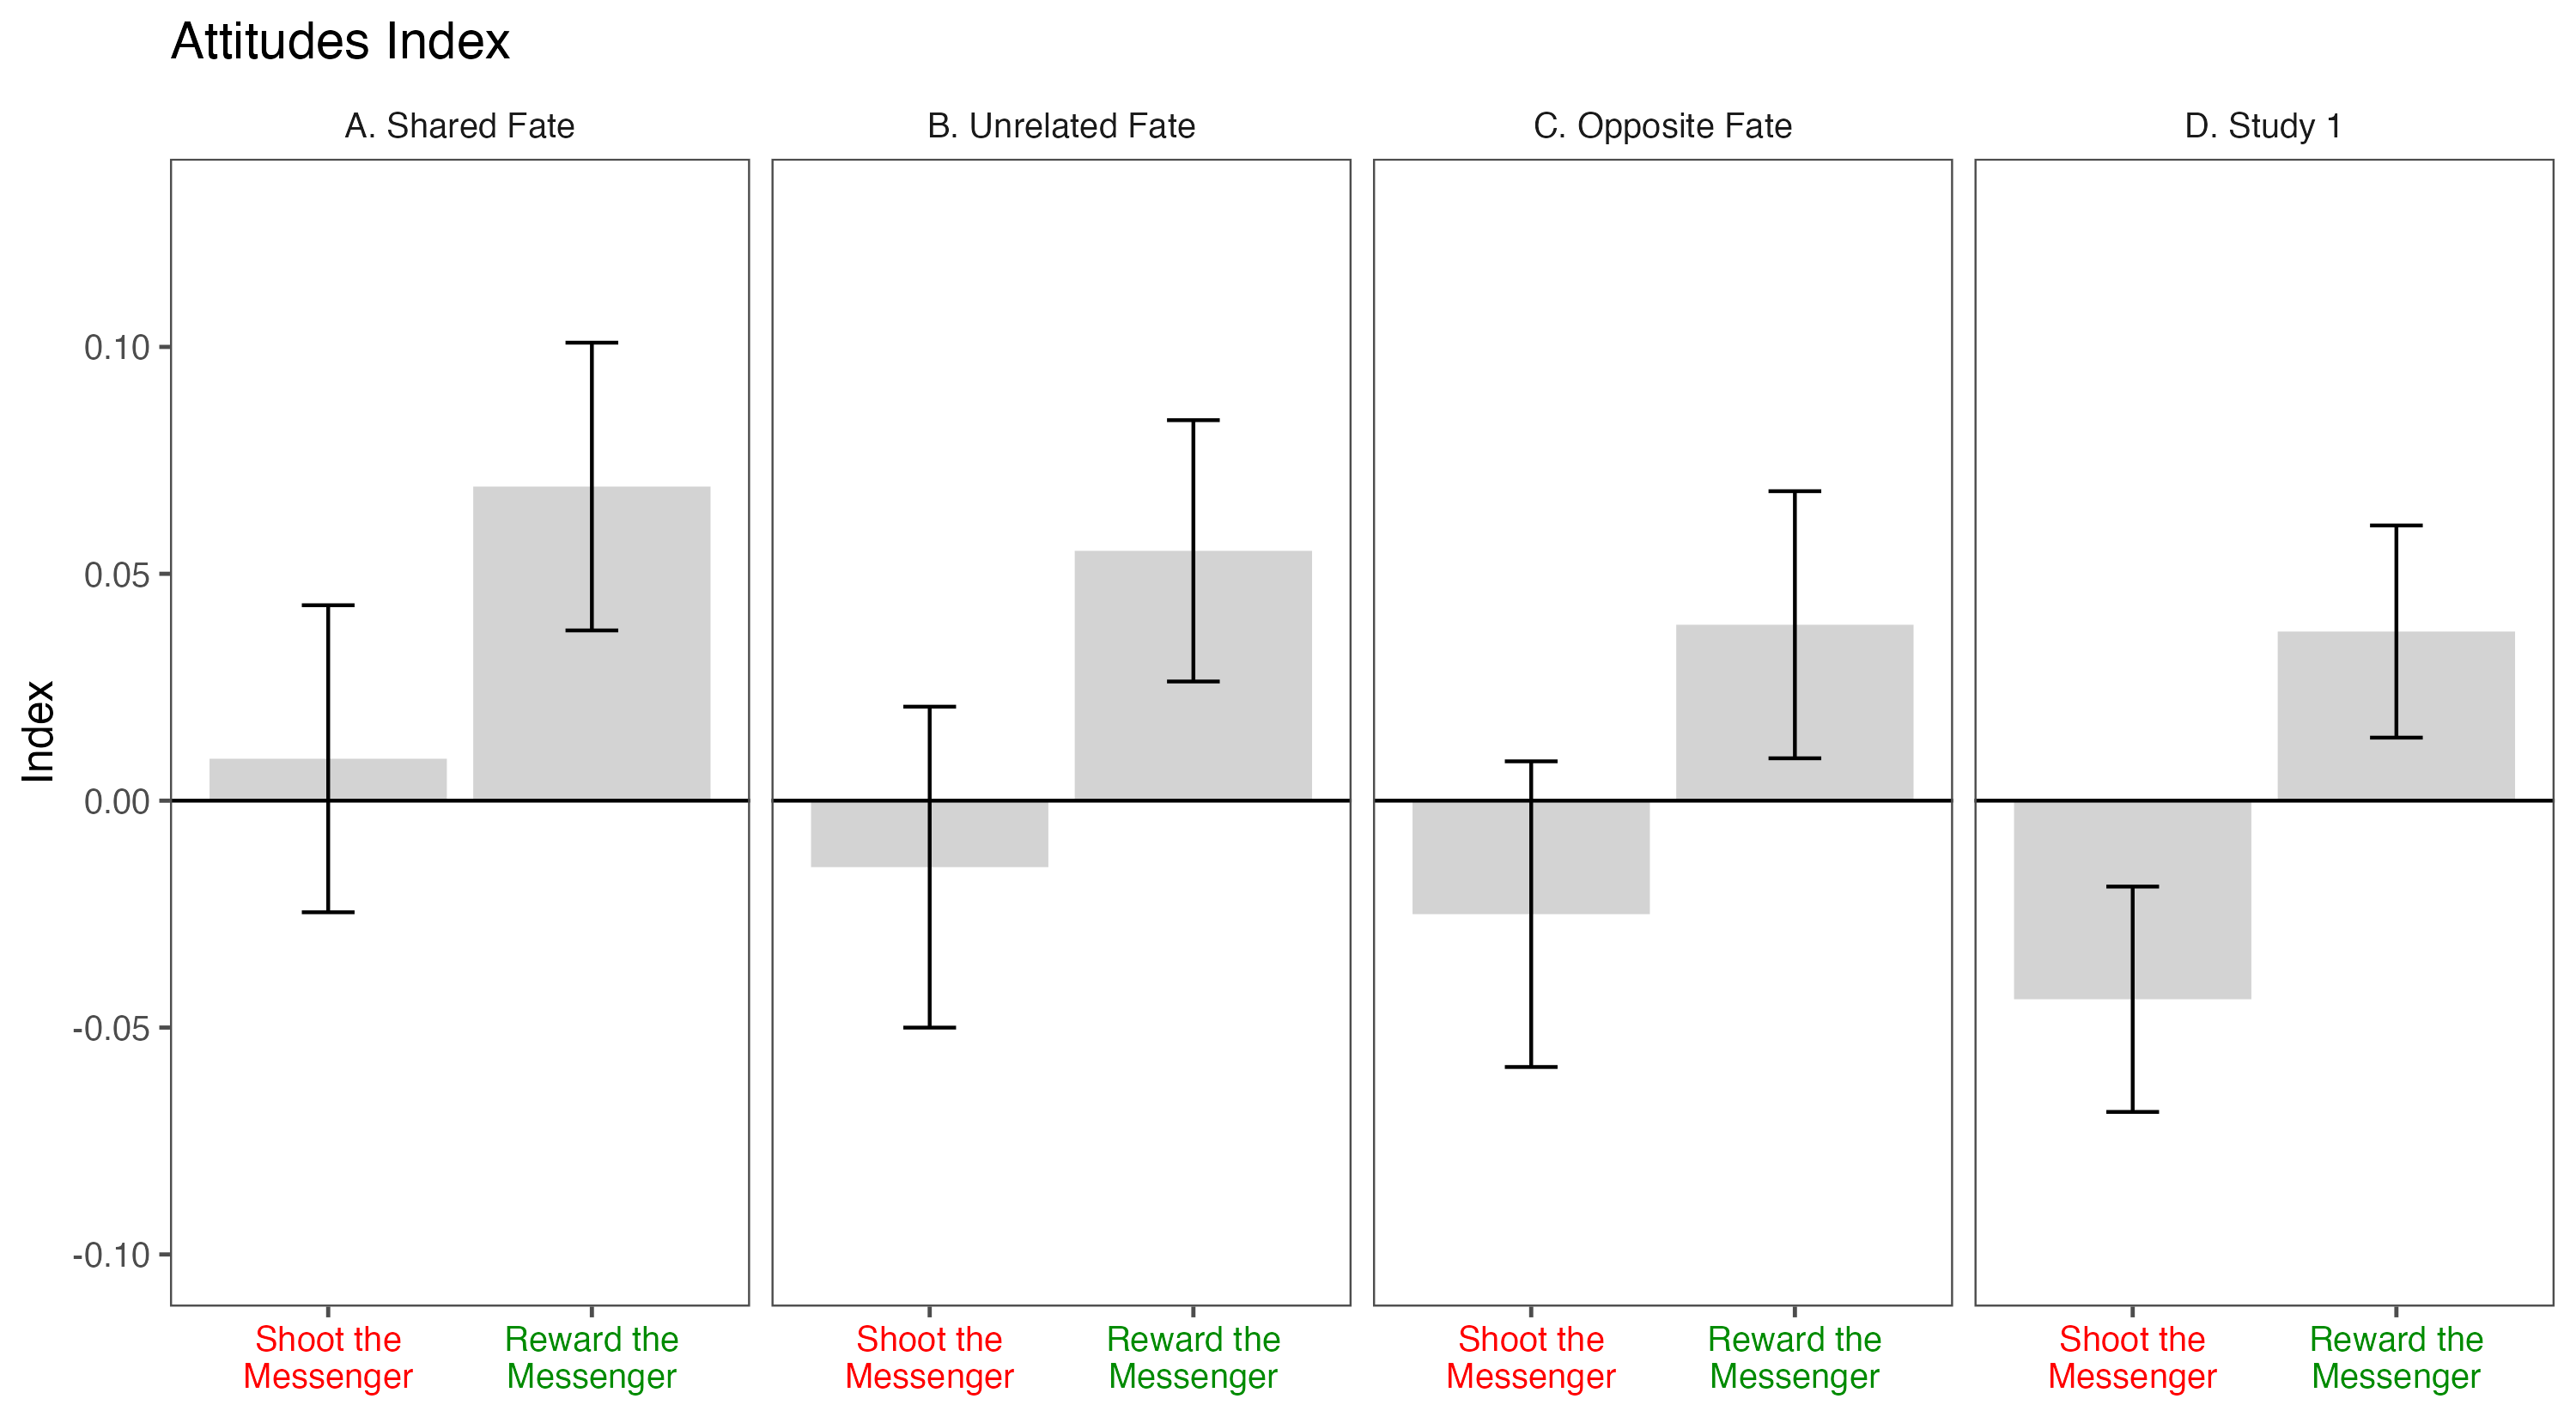
\includegraphics[width=1.0\textwidth]{figures/study2_main_attitude_all.png}
  \caption{Difference in messenger and non-messenger ratings of the Attitudes Index by losing (STM) and winning (RTM) across Unrelated Fate, Shared Fate, Opposite Fate conditions, Study 2. 
  \textit{Note: OLS regression with robust standard errors, with error bars representing 95\% confidence intervals.In the attitudes index, the DV is calculated by averaging the ratings of the trustworthy, nice, likeable, and generous DVs to an index ranging from 0 to 1. The Shared Fate (Panel A), Unrelated Fate (Panel B), and Opposite Fate (Panel C) conditions are when the partner wins when the respondent wins, the partner winning are unrelated to the respondent winning, and the partner wins when the respondent loses, respectively. Study 1 (Panel D) repeats the index measure from Study 1 as a reference, where respondents were not explicitly given the alignment of their partner. The p-values of the test that $RTM = -STM$ are 0.00, 0.08, 0.55, and 0.71, respectively, for the Shared, Unrelated, Opposite Fate conditions, and Study 1. The p-values of the messenger bias are 0.00, 0.00, 0.01, and 0.00, respectively, for the Shared, Unrelated, Opposite Fate conditions, and Study 1.}}
  \label{fig:study2_main_attitude_all}
\end{figure}%
\renewcommand{\baselinestretch}{1.67}%
